\section{Introduction}\label{seg:intro}
Ever since the studies that managed to capture steady-state thermal by Fanger et. al in 1970s\cite{Fanger1970}, the intention to capture the relationship between environmental, personal and other contextual factors against the thermal sensation has been steady and diligent. This has led to many significant findings including understanding thermal comfort can be adaptive\cite{deDear1998Adaptive}, alongside recongnizing comfort is not a single point but a rather acclimatiz-able state. Yet despite the best intention from practitioners and researchers, there appears to be a continuous mismatch between the state-of-the-art research and occupants' complaint that buildings are not `comfortable', leading to an increasing level of interests on how to ensure individual thermal comfort through approaches like personalize thermal comfort models\cite{fang2022data}, individual thermal comfort profiles, etc\cite{ashrafi2022machine}. None of these data-driven models seemed to have truly touched the bottom of the issue of why thermal sensation remains an unsolvable myth to most of these models, regardless however many experimental studies they claimed to have added to some commonly well-known open-source datasets. Aside from a few dedicated studies pointing to the need to correct these datasets before using for machine learning\cite{quintana2024dataset}, very little efforts were dedicated to how could we fill in the missing values for these databases. This led us to question whether we've been recognizing the challenges that are hiding behind the scenes of thermal comfort datasets all along: how much can we trust these open-source datsets? What are the hidden assumptions that sits behind using them, and how do we address their difficiencies? More importantly, what kind of insights can we meaningfully extract from these dataset? 

To address the dual challenges of missing data and physiological realism, we argue that thermal comfort modeling requires a new kind of architecture—one that can simultaneously learn from incomplete data and remain grounded in human physiology. Purely data-driven models, like tree ensembles or standard neural networks, often overfit or “hallucinate” physiologically implausible states, while traditional imputation methods lack robustness in high-missingness regimes. Likewise, while physics-informed neural networks \gls{pinn} have shown promise in enforcing known biophysical relationships, they are rarely applied to settings with heavy missingness. Our insight is to combine the strength of probabilistic imputation through a variational autoencoder (VAE) with the realism enforced by physiological constraints, yielding a hybrid PINN-VAE architecture tailored for occupant-centric thermal modeling.

% Where would I squeeze in the bit on BMR...? Now getting a bit confused here.
To test this novel architecture, we combined two of the largest open-source steady-state thermal sensation datasets that are available, notably the ASHRAE Global Thermal Comfort Database II (ASHRAE II from hereon), and the Chinese Thermal Comfort Datsets (Chinese DB from hereon)\cite{foldvary2018ashrae,yang2023chinese}. Upon harmonizing these datasets, we noticed a significant amount (33\%) of fields are null-valued. Crucially, before robust imputation techniques like Variational Autoencoders (\gls{vae}) can be confidently applied, the nature of this missingness must be understood. The prerequisite for VAE-based imputation is that the data satisfy the Missing At Random (MAR) assumption, so we first confirmed MAR holds for our datasets before employing the VAE \cite{nazabal2020handling}. As VAE alone does not have any knowledge towards each of fields' actual limitations, we implemented special cost functions to ensure the imputation process in conjunction with the prediction of our thermal sensation can be constrained via custom loss functions: both on the existing distribution of field-specific distribution\cite{Raissi2019PINN}, but also on intermediate outputs such as $T_{skin}$, $T_{core}$ and $\omega$. To ensure that we put an extra emphasis on ensuring that our PINN-VAE model accounts the personal profiles that we fit better, we explicitly added a PPI header to the model architecture to assess between \gls{pinn}, \gls{pinnvae} and \gls{pvp} which performs better against our purely data-driven benchmark, an lightgbm alternative.

Upon assembling the cross-validated prediction results from all models, we noticed our PINN-VAE models consistently fared better than its lightgbm alternatives\cite{ke2017lightgbm} around neutral-thermal-sensation targets. As the thermal-neutral state accounts to almost 50\% of all of the thermal sensation collected, these models were outperformiung lightgbm families consistently around 9-10\% drop of \gls{rms} and \gls{mae} (numbers fluctuated based on which variant of PINN-VAE was tested during our ablation efforts to identify the root cause of proposed architecture improvements. We observed these performance uplift not only against the vanilla (without any \gls{bmr} even) lightgbm, but also the lightgbm that went through 10-fold cross validation on their imputed data. This led us to believe that not only is the effort of suggesting a framework to impute missing dataset values are valuable, the PINN-VAE architecture, with or without PPI, offers consistent performance gains over baselines.

Our approach has demonstrated that 1. generative models like VAE can lead to sufficient imputation of missing values in a historical archival dataset that was compiled over a long period of time as a novel implementation of this new framework, 2. physiological constraints implemented on the data allows the model to better self-regulate. %Cite the skin and core temperature imputation results here, as the T_skin and T_core originally is pretty problematic.
3. even historical data that has missing values, so long as their \gls{mar}-validity can be established, can be filled with our suggested framework - especially as the physiological constraints we implemented are only constraints, which can be easily generalized to problems beyond the scope of thermal comfort studies. 

The remainder of this paper will follow the following road map shown in this conceptual schematic on its workflow. We first begin with harmonizing the QC databases, identifying the level of missing data at different `rungs' to better assess how much of the data is missing and by what year in the data preparation phase, and then pass them on to test their MAR validity to confirm that we are a go to prepare the data for PINN-VAE. We then constructed VAE by leveraging the data to train three different models, VAE, PINN-VAE and PINN-VAE-\gls{ppi}. At this stage an alternate variate, PPI-analytic is also extracted where the final weights from the PINN-VAE-PPI is frozen and extracted as a potential guide to how personal identifiers can be leveraged by these models. We then compare our model performance by contrasting the VAE, VAE-PINN, PPI-Analytic, with a \gls{lightgbm} baseline both on a global level, `rung'-specifc level, and then slice level. This includes evaluating the thermal-neurtal band, i.e. [-0.5,0.5] thermal sensation as targets as well.

\begin{figure}
    \centering
    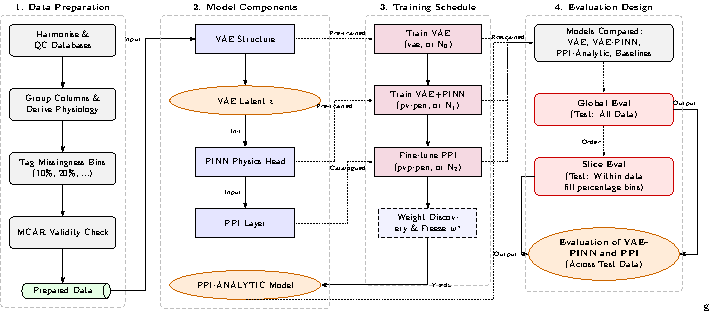
\includegraphics[width=0.95\linewidth]{fig/PINN_VAE_Diagram.pdf}
    \caption{Workflow diagram of current paper: An Overview}
    \label{fig:workflow}
\end{figure}

%Some uplifting sentences
We believe this approach of data imputation alongside the model architecture provides a unique and novel angle to approach the simulation of a physiology-based experimental historical dataset. For that matter we believe we are presenting a significant advancement that warrants dissemination.

